\documentclass{article}
\usepackage{tikz}
\usepackage{tkz-euclide}
\definecolor{darkgreen}{RGB}{0,192,0}
\title{Cartesian closed categories and the price of eggs}
\author{Jane Doe}
\date{September 1994}
\begin{document}

	\begin{figure}
		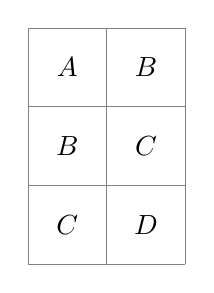
\begin{tikzpicture}
			\draw[step=1cm,gray,very thin] (0,0) grid (2,-3);
			\draw (0.5,-0.5) node {$A$};
			\draw (1.5,-0.5) node {$B$};
			\draw (0.5,-1.5) node {$B$};
			\draw (1.5,-1.5) node {$C$};
			\draw (0.5,-2.5) node {$C$};
			\draw (1.5,-2.5) node {$D$};			
		\end{tikzpicture}
		\hspace{5mm}
		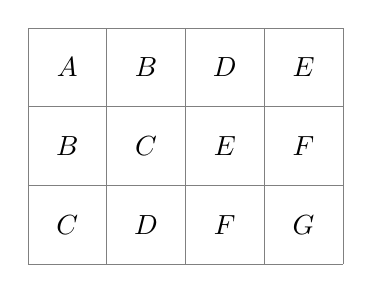
\begin{tikzpicture}
			\draw[step=1cm,gray,very thin] (0,0) grid (4,-3);
			\draw (0.5,-0.5) node {$A$};
			\draw (1.5,-0.5) node {$B$};
			\draw (0.5,-1.5) node {$B$};
			\draw (1.5,-1.5) node {$C$};
			\draw (0.5,-2.5) node {$C$};
			\draw (1.5,-2.5) node {$D$};	

			\draw (2.5,-0.5) node {$D$};
			\draw (3.5,-0.5) node {$E$};
			\draw (2.5,-1.5) node {$E$};
			\draw (3.5,-1.5) node {$F$};
			\draw (2.5,-2.5) node {$F$};
			\draw (3.5,-2.5) node {$G$};					
		\end{tikzpicture}
		\caption{\textit{Left:} A cubic curve with control points $A,B,C,D$ encoded in a 2d texture that is $(2,3)$ in size.  \textit{Right:} Two piecewise curves encoded in a 2d texture that is $(4,3)$ in size.  The control points for the first curve are $A,B,C,D$ and the control points for the second curve are $D,E,F,G$.}	
		\label{fig:texlayeout1d}
	\end{figure}	

\end{document}